\documentclass[11pt,letterpaper]{article}
\PassOptionsToPackage{hyphens}{url}
\usepackage[margin=.83in,top=.8in,bottom=.8in,headheight=15pt]{geometry}
\usepackage[T1]{fontenc}
\usepackage{lmodern,amsmath,amssymb,mathtools,bm,booktabs,array,graphicx,tikz}
\usetikzlibrary{arrows.meta,positioning,calc,decorations.pathreplacing,patterns}
\definecolor{ink}{HTML}{17344D}\definecolor{accent}{HTML}{087E8B}\definecolor{pale}{HTML}{EDF5F5}\definecolor{gold}{HTML}{AD6B19}
\providecommand{\dd}{\,\mathrm{d}}\providecommand{\R}{\mathbb{R}}
\providecommand{\E}{\mathbb{E}}\providecommand{\Var}{\operatorname{Var}}
\providecommand{\Cov}{\operatorname{Cov}}\providecommand{\diag}{\operatorname{diag}}
\providecommand{\norm}[1]{\left\lVert#1\right\rVert}
\providecommand{\abs}[1]{\left|#1\right|}
\usepackage{microtype,hyperref,fancyhdr,enumitem,amsthm,sectsty,needspace}
\allsectionsfont{\raggedright}
\hypersetup{colorlinks=true,linkcolor=ink,urlcolor=accent,pdfauthor={Zan Ahmad},pdftitle={Fetal pathways and signed junction balances / Lecture notes}}
\setlength{\parindent}{0pt}\setlength{\parskip}{6pt}\linespread{1.07}
\setlist{itemsep=3pt,topsep=4pt,leftmargin=*}
\emergencystretch=2em\clubpenalty=10000\widowpenalty=10000
\pagestyle{fancy}\fancyhf{}\fancyhead[L]{\small Mathematical Cardiology}\fancyhead[R]{\small Lecture 7}
\fancyfoot[L]{\footnotesize Zan Ahmad}\fancyfoot[R]{\footnotesize\thepage}\renewcommand{\headrulewidth}{.3pt}
\newtheorem{proposition}{Proposition}\newtheorem{theorem}{Theorem}\newtheorem{lemma}{Lemma}
\theoremstyle{definition}\newtheorem{definition}{Definition}\newtheorem{example}{Example}
\numberwithin{equation}{section}
\begin{document}
{\small\scshape Mathematical Cardiology\hfill Lecture 7}\par\medskip
{\raggedright\hyphenpenalty=10000\exhyphenpenalty=10000\LARGE\bfseries\color{ink} Fetal pathways and signed junction balances\par}\medskip
{\small Lecture notes}\par\bigskip
A circulation diagram is useful only after its arrows have been given a mathematical meaning. Some arrows indicate a permitted direction; others merely specify which direction is counted as positive. The fetal circulation makes this distinction unavoidable. We shall retain two shunts, write the junction balances, and then use local pressure laws to decide which flows can reverse.

\section{Interpretation of the grouped network}
\hypertarget{note-interpretation-of-the-grouped-network}{}\label{note:interpretation-of-the-grouped-network}
{\small \href{slides.html\#frame=two-shunts-change-the-routes-figure\&step=1}{Slides for this section}}\par
The placenta provides fetal gas exchange. Maternal and fetal blood approach one another across an exchange interface; they are not a single freely mixed stream. Oxygenated placental return travels in the umbilical vein. Some of this return passes through the liver and some through the ductus venosus toward the inferior vena cava. The umbilical arteries carry fetal blood back toward the placenta. Vessel names therefore describe direction relative to the heart, not a universal oxygen-content rule.

We group the body and placenta into one systemic route, and group each ventricle with its major outgoing vessel. Two additional connections remain explicit: the foramen ovale between right and left atria, and the ductus arteriosus between pulmonary artery and aorta. The fetal lungs have relatively high resistance but are still perfused; ``little pulmonary flow'' must not be replaced by ``no pulmonary flow.'' These groupings omit liver routing and oxygen streaming. They will support flow balances, not a detailed prediction of oxygen delivered to each organ.

Let $Q_R$ and $Q_L$ denote right- and left-pump outputs, $Q_p$ pulmonary flow, and $Q_s$ the grouped systemic flow. Count $Q_d$ as positive from pulmonary artery to aorta and $Q_f$ as positive from right to left atrium. The sign definitions are part of the model. They must be fixed before any pressure difference is inserted.
\begin{center}\begin{minipage}{.98\linewidth}\centering
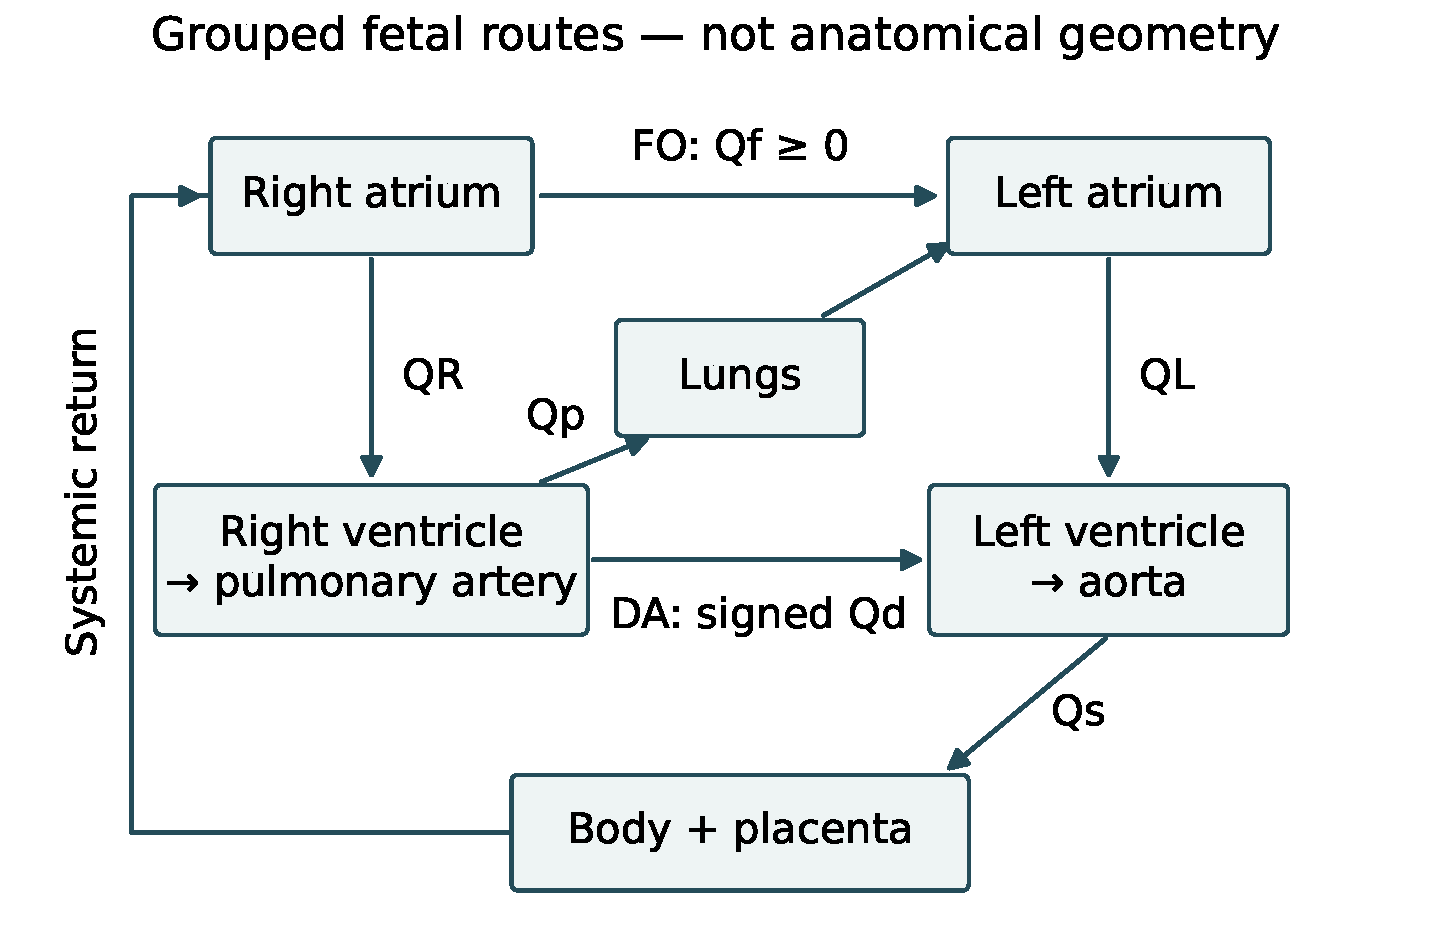
\includegraphics[width=.96\linewidth,height=.57\textheight,keepaspectratio]{fetal-routes.pdf}\par\smallskip
{\small Original non-anatomical route graph. FO: foramen ovale; DA: ductus arteriosus. Body and placenta are grouped for flow balance; umbilical vessels and ductus venosus are described in the notes, not explicitly modeled.}
\end{minipage}\end{center}
\section{Four junctions, three independent equations}
\hypertarget{note-four-junctions-three-independent-equations}{}\label{note:four-junctions-three-independent-equations}
{\small \href{slides.html\#frame=at-the-pulmonary-artery\&step=1}{Slides for this section}}\par
At the pulmonary-artery junction, right-pump output divides into pulmonary and ductus flow. At the left atrium, pulmonary and foramen flows combine. At the aortic junction, left-pump and ductus flows combine. Thus
\begin{align}
Q_R&=Q_p+Q_d,\label{eq:fetal-right}\\
Q_L&=Q_p+Q_f,\label{eq:fetal-left}\\
Q_s&=Q_L+Q_d.\label{eq:fetal-aorta}
\end{align}
The right-atrial balance is $Q_s=Q_R+Q_f$. It follows from the first three equations:
\[Q_L+Q_d=(Q_p+Q_f)+Q_d=(Q_p+Q_d)+Q_f=Q_R+Q_f.
\]
This dependence is an instance of conservation. Summing all junction balances cancels every internal flow because it leaves one junction and enters another. Counting four equations does not therefore give four independent constraints.

For $Q_p=100$, $Q_d=50$ and $Q_f=40\,\mathrm{mL/min}$, the balances give $Q_R=150$, $Q_L=140$ and $Q_s=190\,\mathrm{mL/min}$. The pump outputs need not equal each other or equal pulmonary flow in this shunted network. In particular, imposing the adult series-circulation equality $Q_R=Q_L=Q_p=Q_s$ would silently erase the shunts.
\section{A reversible ductus and a one-way foramen}
\hypertarget{note-a-reversible-ductus-and-a-one-way-foramen}{}\label{note:a-reversible-ductus-and-a-one-way-foramen}
{\small \href{slides.html\#frame=an-open-ductus-can-reverse-figure\&step=1}{Slides for this section}}\par
For an open ductus with positive resistance $R_d$, take
\begin{equation}Q_d=\frac{P_{pa}-P_{ao}}{R_d}.\end{equation}
This is a signed linear law. With $R_d=0.1\,\mathrm{mmHg\,min/mL}$, pulmonary and aortic pressures $30$ and $25\,\mathrm{mmHg}$ give $Q_d=50\,\mathrm{mL/min}$. Pressures $20$ and $30$ instead give $Q_d=-100\,\mathrm{mL/min}$: the actual direction is from aorta to pulmonary artery. Negative flow is a meaningful result, not a negative volume of blood.

The foramen surrogate uses a different law:
\begin{equation}Q_f=\frac{\max(P_{RA}-P_{LA},0)}{R_f},\qquad R_f>0.\end{equation}
For $R_f=0.05\,\mathrm{mmHg\,min/mL}$, atrial pressures $6$ and $4\,\mathrm{mmHg}$ give $Q_f=40\,\mathrm{mL/min}$. Reversing the pressure ordering to $4$ and $7$ produces zero flow. A negative pressure difference does not generate reverse flow under this one-way rule. The finite forward resistance used here also differs from an ideal zero-resistance valve: forward flow can coexist with a positive pressure drop.

A closed ductus has zero conductance, $G_d=0$, so $Q_d=G_d(P_{pa}-P_{ao})=0$. Setting resistance to zero would describe an entirely different limit. Equal pressures also produce zero ductus flow even when its conductance is positive; a zero flow observation alone cannot demonstrate anatomical closure.
\begin{center}\begin{minipage}{.98\linewidth}\centering
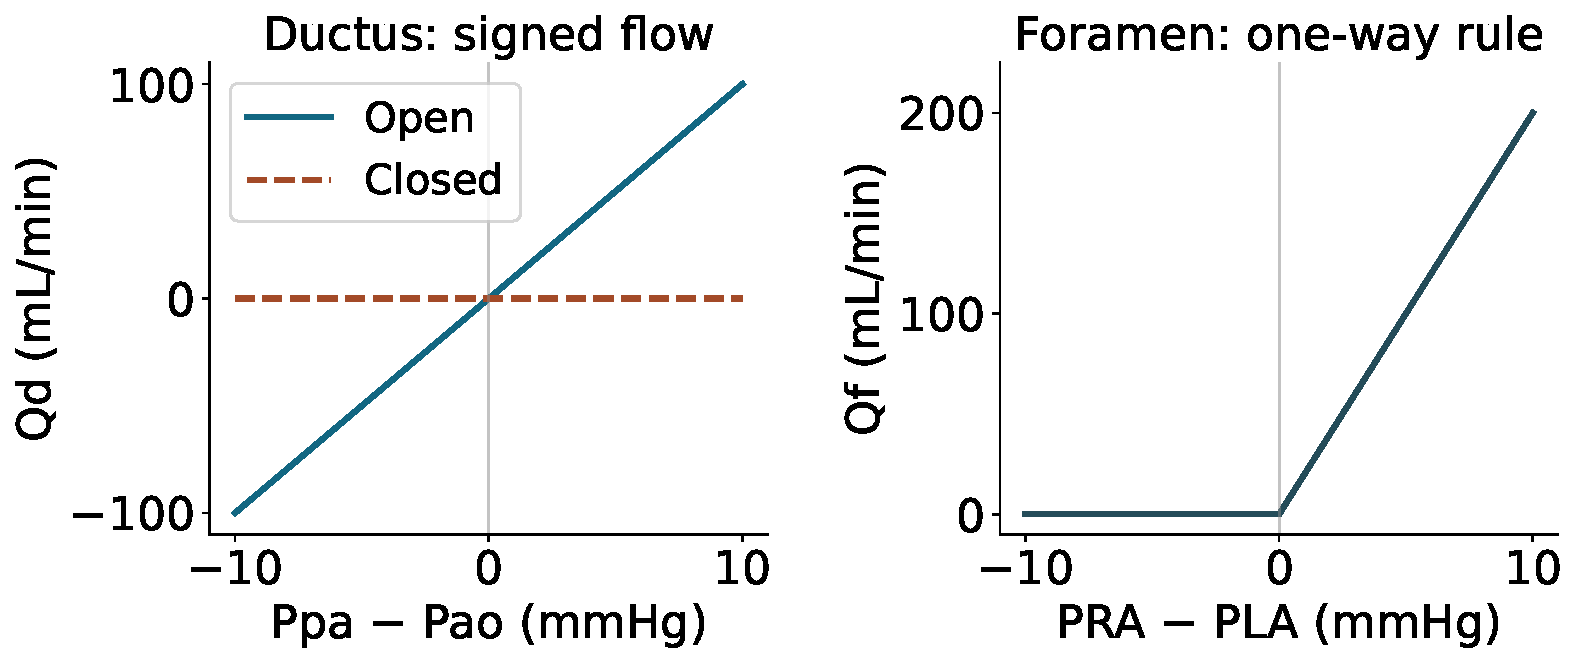
\includegraphics[width=.96\linewidth,height=.57\textheight,keepaspectratio]{shunt-rules.pdf}\par\smallskip
{\small Open ductus Rd =\allowbreak{} 0.1 and finite forward foramen Rf =\allowbreak{} 0.05 mmHg min/mL. A declared closed ductus has zero conductance. These are local rules at prescribed pressures.}
\end{minipage}\end{center}
\section{Reversal still obeys conservation}
\hypertarget{note-reversal-still-obeys-conservation}{}\label{note:reversal-still-obeys-conservation}
{\small \href{slides.html\#frame=reversed-flow-enters-the-pulmonary-junction\&step=1}{Slides for this section}}\par
Suppose $Q_p=300$, $Q_d=-100$ and $Q_f=0\,\mathrm{mL/min}$. Then
\[Q_R=300-100=200,\qquad Q_L=300,\qquad Q_s=300-100=200.
\]
The pulmonary flow exceeds the right-pump output because an additional $100\,\mathrm{mL/min}$ arrives from the aorta through the reversed ductus. At the aorta, the left pump provides $300$, of which $100$ leaves through the ductus and $200$ enters the grouped systemic route. The same signed number works in both balances because it represents one shared connection.

An alternative algebraic view collects $q=(Q_R,Q_L,Q_p,Q_s,Q_d,Q_f)^T$ and writes
\begin{equation}
\begin{pmatrix}
1&0&-1&0&-1&0\\
0&1&-1&0&0&-1\\
0&-1&0&1&-1&0
\end{pmatrix}q=0.
\end{equation}
This matrix is simply a compact list of the three balances; each row can be read without any matrix methods. Six flow unknowns and three independent balance equations leave three degrees of freedom. Pressure laws and the rest of the circulation must supply further information. In the companion, local pressures and illustrative pulmonary flows are prescribed. It is not a solved whole-circulation pressure network, and arbitrary prescribed values need not all fit a complete physiological model.
\section{Changing the network at birth}
\hypertarget{note-changing-the-network-at-birth}{}\label{note:changing-the-network-at-birth}
{\small \href{slides.html\#frame=the-transition-changes-both-pressures-and-routes\&step=1}{Slides for this section}}\par
Lung aeration changes pulmonary vascular conditions, and separation from the placenta removes a vascular route. Changing atrial and arterial pressures can alter the shunt flows even before the anatomy has fully changed. Under the signed ductus law, a pressure reversal can reverse flow while the ductus remains open. Under the one-way foramen rule, a sufficiently high left-atrial pressure suppresses forward flow. Functional absence of flow and anatomical closure are distinct statements.

If both shunts are set to zero and the same grouped steady balances are retained, equations \eqref{eq:fetal-right}--\eqref{eq:fetal-aorta} reduce to $Q_R=Q_p=Q_L=Q_s$. The familiar series relation reappears as a limiting case. One cannot obtain that case by deleting arrows while retaining the former numerical flows: the junction balances must be solved again. Nor can the local rules predict the timing of the postnatal transition. Such a prediction would require evolving resistances, chamber behavior and an account of the physical closure mechanisms. The value of the small network is that it makes these missing ingredients identifiable.
\bigskip
\section*{Exercises}
\par\noindent\begin{minipage}{\linewidth}
\subsection*{MC07-E1. Keep the shunts straight}
Use positive ductus flow from pulmonary artery to aorta with Rd =\allowbreak{} 0.2 mmHg min/mL, and foramen flow from right to left atrium with forward Rf =\allowbreak{} 0.1.

\textbf{a} Name the two anatomical endpoints of each connection.

\end{minipage}\par\medskip
\textbf{b} Find ductus flow when Ppa =\allowbreak{} 24 and Pao =\allowbreak{} 30 mmHg. State physical direction.

\textbf{c} Find foramen flow for PRA =\allowbreak{} 5 and PLA =\allowbreak{} 8 mmHg using the one-way surrogate; explain why zero does not prove anatomical closure.

\par\noindent\begin{minipage}{\linewidth}
\subsection*{MC07-E2. Audit a junction table}
A prescribed state has Qp =\allowbreak{} 180, Qd =\allowbreak{} 60 and Qf =\allowbreak{} 20 mL/min.

\textbf{a} Calculate QR and QL.

\end{minipage}\par\medskip
\textbf{b} Find Qs in two independent ways.

\textbf{c} A student erases both shunt flows but keeps QR =\allowbreak{} 240 and QL =\allowbreak{} 200. Explain the inconsistency and give one consistent closed-shunt state.

\par\noindent\begin{minipage}{\linewidth}
\subsection*{MC07-E3. Interpret a birth-transition claim}
A caption says: ``The ductus flow becomes zero, proving that the newborn transition is complete.''

\textbf{a} Give two distinct modeled reasons for zero ductus flow.

\end{minipage}\par\medskip
\textbf{b} Name two physiological changes beyond a ductus edge law and identify the source of oxygen uptake before birth.

\textbf{c} Rewrite the caption as a bounded claim and propose an observation needed to distinguish the two zero-flow explanations.

\section*{References}
\noindent\begin{minipage}{\linewidth}
Zan Ahmad, Fall 2023 HEART syllabus. Public PDF pp. 1--2, Course Topics and Course Expectations; editable syllabus pp. 2--3, project requirements.

\end{minipage}\par\medskip
\noindent\begin{minipage}{\linewidth}
Hoppensteadt and Peskin, Modeling and Simulation in Medicine and the Life Sciences, second edition. Printed pp. 28--30; PDF pp. 41--43, section 1.10, fetal shunt topology and steady junction balances.

\end{minipage}\par\medskip
\noindent\begin{minipage}{\linewidth}
American Heart Association, Fetal Circulation. Fetal pathways and changes after birth.

\url{https://www.heart.org/en/health-topics/congenital-heart-defects/symptoms--diagnosis-of-congenital-heart-defects/fetal-circulation}
\end{minipage}\par\medskip
\noindent\begin{minipage}{\linewidth}
US Food and Drug Administration, Pediatric Advisory Committee briefing, 2023. Section 3.1.1, Fetal circulation/physiology.

\url{https://www.fda.gov/media/172183/download}
\end{minipage}\par\medskip
\end{document}
